\documentclass{beamer}

\usepackage{afit-beamer-template}
\graphicspath{{diagrams/},{figure/},{afit-images/}} 

\usepackage{booktabs}
\usepackage{color}

% Command line/terminal-like environment
% Todo tag
\newcommand{\tbd}[1]{{\color{red} TBD: #1}}



\title[Title Desert]{Malicious Traffic Detection through Internet Protocol Address Hopping}
\author[Morehart]{2Lt~Ryan~A.~Morehart}
\institute[AFIT/ENG]{%
  Department of Electrical \& Computer Engineering
  Air Force Institute of Technology%
}

\date[February 2013]{21 February 2013}

\begin{document}

\begin{frame}
  \titlepage
\end{frame}

\section{Acknowledgments}
\begin{frame}
	\frametitle{Acknowledgments}
	\begin{itemize}
	\item Thesis committee
		\begin{itemize}
		\item Dr. Barry Mullins (advisor)
		\item Dr. Rusty Baldwin
		\item Dr. Timothy Lacey
		\end{itemize}
	\end{itemize}
\end{frame}

\section{Overview}
\begin{frame}
	\frametitle{Overview}
	\tableofcontents
\end{frame}

\section{Motivation}
\begin{frame}
	\frametitle{Motivation}

	\begin{itemize}
	\item Networks are critical to many aspects of the modern military and corporations
	\item Protecting these is a huge concern
	\item Traditional network defenses (firewalls, IDSs) help
	\item Interest has increased in more dynamic forms of protection
		\begin{itemize}
		\item Reputation/trust-based security
		\item Machine learning
		\item Network address space randomization (``IP hopping'')
		\end{itemize}
	\end{itemize}
\end{frame}

\section{Background}
\begin{frame}
	\frametitle{Background - IP Hopping}
	\begin{itemize}
	\item More formally part of ``network address space randomization''
	\item IP hopping involves systems changing IP addresses on a periodic basis
		\begin{itemize}
		\item No pattern to outside observer
		\item ``Hops'' typically chosen based on a shared secret
		\item Often coupled with encryption between IP hopping systems
		\end{itemize}
	\item Presents a moving target to an outside attacker
		\begin{itemize}
		\item Obfuscates true sender of sniffed traffic
		\item Network maps established by attacker change frequently
		\end{itemize}
	\item Two basic approaches exist:
		\begin{itemize}
		\item End point-based hopping
		\item Gateway-based hopping
		\end{itemize}
	\end{itemize}
\end{frame}

\begin{frame}
	\frametitle{Background - Gateway Hopping}
	In gateway-based hopping, a system in front of the network transforms
	packets entering and leaving.
	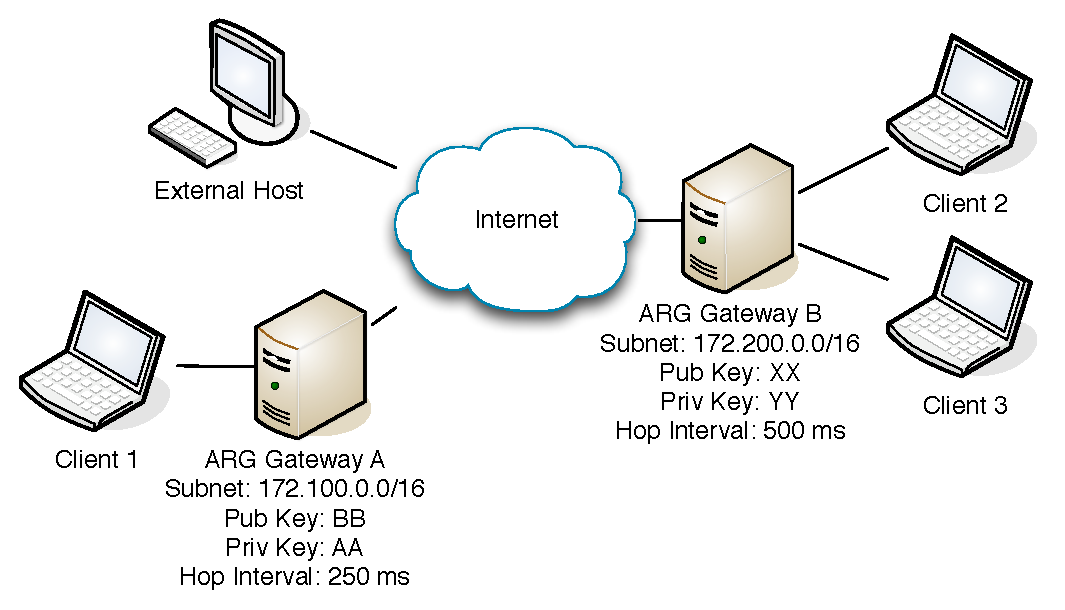
\includegraphics[width=1\textwidth]{arg_concept_network}
\end{frame}

\begin{frame}
	\frametitle{Background - Routing}

	% Build 1
	\begin{onlyenv}<1>
	Hierarchical nature of IP routing allows IP hopping to work
	\begin{figure}
	\centering
	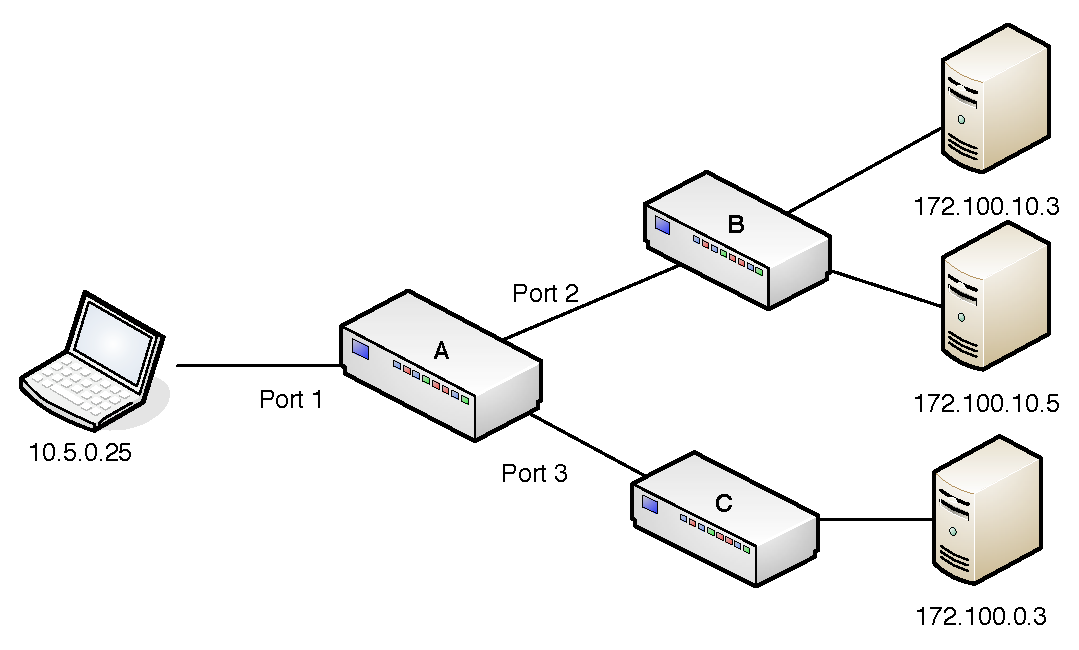
\includegraphics[height=.5\textheight]{routing_example_network}
	\end{figure}
	\end{onlyenv}

	% Build 2
	\begin{onlyenv}<2>
	\scriptsize{%
	\begin{table}
	\centering
	\begin{tabular}{rccc}
	\toprule
	 & \textbf{IP} & \textbf{Mask} & \textbf{Interface}\\
	\hline
	1 & 10.5.0.25 & 255.255.0.0 & Port 1\\
	2 & 172.100.10.0 & 255.255.255.0 & Port 2\\
	3 & 172.100.0.0 & 255.255.0.0 & Port 3\\
	\bottomrule
	\end{tabular}
	\end{table}%
	}
	\vspace{-25pt}
	\begin{figure}
	\centering
	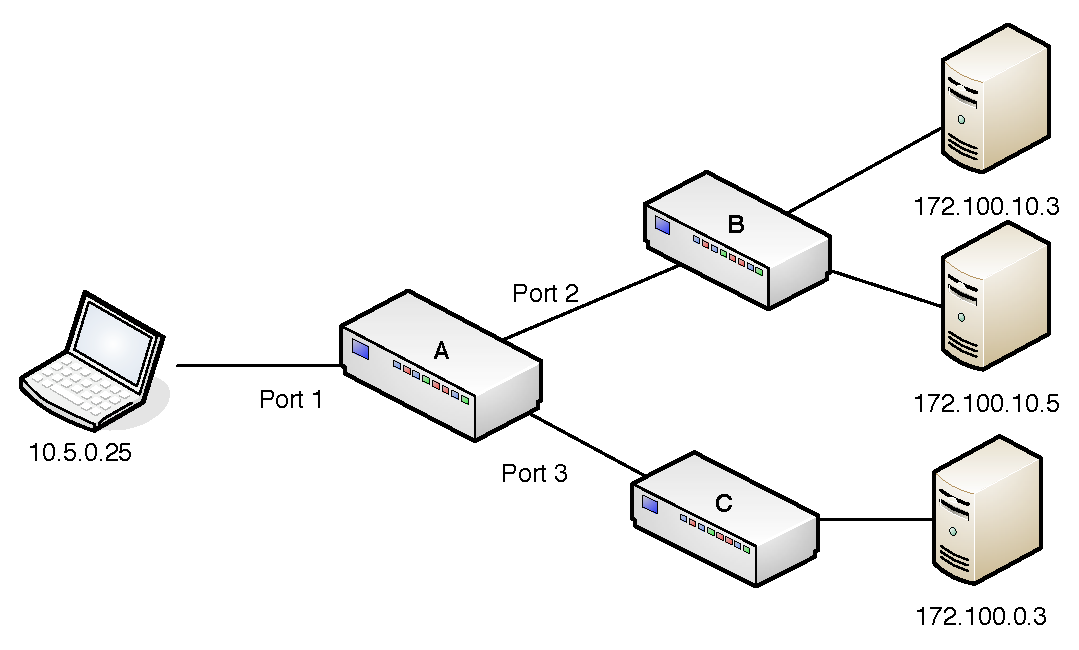
\includegraphics[height=.6\textheight]{routing_example_network}
	\end{figure}
	\end{onlyenv}
\end{frame}

\section{Goals and Approach Overview}
\begin{frame}
	\frametitle{Goals}

	\begin{itemize}
	\item Study effectiveness of IP hopping in classifying traffic
	\item Approach:
		\begin{itemize}
		\item Develop custom IP hopping solution combining previous research to meet military network needs
		\item Create test network
		\end{itemize}
	\end{itemize}
\end{frame}

\section{Implementation}
\begin{frame}
	\frametitle{Implementation - Requirements}

	\begin{itemize}
	\item Security over any network (including confidentiality)
	\item Utilizes existing commercial infrastructure
	\item Must not terminate connections unnecessarily
	\item Easily deployable onto the network
		\begin{itemize}
		\item No hardware changes, minimal software configuration changes
		\item Allow use with legacy systems
		\end{itemize}
	\end{itemize}
\end{frame}

\begin{frame}
	\frametitle{Implementation - Features}

	\begin{itemize}
	\item Gateway-based
	\item Capable of hopping many times per second
	\item No configuration changes needed by the hosts inside
	\item Fully encrypted and authenticated packets between ARG-protected networks
	\item No connection drops across hops
	\item Easy configuration for each gateway
		\begin{itemize}
		\item Self: private key, hop interval, IP range
		\item Others: public key, IP range
		\end{itemize}
	\end{itemize}
\end{frame}

\begin{frame}
	\frametitle{Implementation - Architecture}

	\begin{columns}
	\begin{column}{.45\textwidth}
		Three components
		\begin{itemize}
		\item \textbf{Director} - Receives incoming packets and decides how to handle
		\item \textbf{Hopper} - Maintains gateway information
		\item \textbf{Network Address Translator (NAT)} - Handles external connections
		\end{itemize}
	\end{column}
	\begin{column}{.55\textwidth}
		\begin{figure}
		\includegraphics[width=\textwidth]{flow_director}
		\end{figure}
	\end{column}
	\end{columns}
\end{frame}

\section{Methodology}
\begin{frame}
	\frametitle{Methodology - Research Questions}

	\begin{itemize}
	\item Does ARG classify traffic correctly? What percentage of false positives (valid packets blocked) and false negatives (invalid traffic allowed through) does it introduce?
	\item What is the maximum packet rate and throughput ARG can support?
	\item What is the minimum supportable time between hops? How does latency affect this?
	\item Is ARG stable when presented with corrupt, malformed, or replayed packets?
	\end{itemize}
\end{frame}

\begin{frame}
	\frametitle{Methodology - Test Network}

	\begin{itemize}
	\item 7 physical systems on 4 VLANs
	\item Artificial latency introduced via \texttt{tc}
	\item Traffic generators used for tests
	\end{itemize}
	
	\vspace{-15pt}
	\begin{figure}
	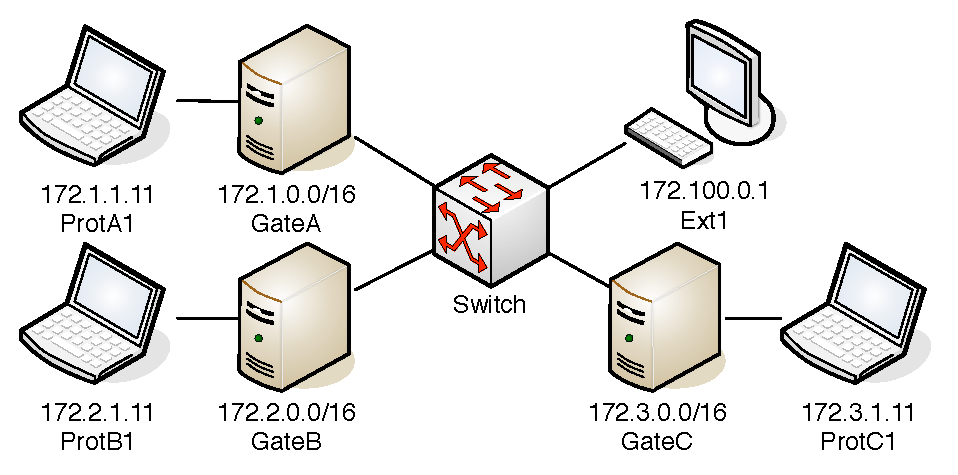
\includegraphics[width=\textwidth]{thesis_network}
	\end{figure}
\end{frame}

\begin{frame}
	\frametitle{Methodology - Metrics}
	\begin{itemize}
	\item Percentage of invalid packets accepted
		\begin{itemize}
		\item ``Invalid'' traffic should \textit{not} be allowed in by ARG
		\end{itemize}
	\item Percentage of valid packets rejected
		\begin{itemize}
		\item ``Valid'' traffic should be allowed in by ARG
		\end{itemize}
	\item Types of rejections seen
	\item Kilobits per second of traffic
	\end{itemize}
\end{frame}

\begin{frame}
	\frametitle{Methodology - Factors}

	\begin{itemize}
	\item Hop interval (ms)
		\begin{itemize}
		\item Time between IP address changes
		\end{itemize}
	\item Round-trip Latency (ms)\\
		\begin{itemize}
		\item Artificial latency 
		\end{itemize}
	\item Packet delay (s)\\
		\begin{itemize}
		\item Time between sends from the traffic generators
		\end{itemize}
	\item Traffic direction and type\\
		\begin{itemize}
		\item Traffic flows
		\end{itemize}
	\end{itemize}
\end{frame}

\begin{frame}
	\frametitle{Methodology - Traffic Flows}
	
	\vspace{-15pt}

	\begin{overprint}
	\onslide<1>
		\begin{columns}
		\begin{column}{.5\textwidth}
			\begin{figure}
			\caption{Traffic Flow 0}
			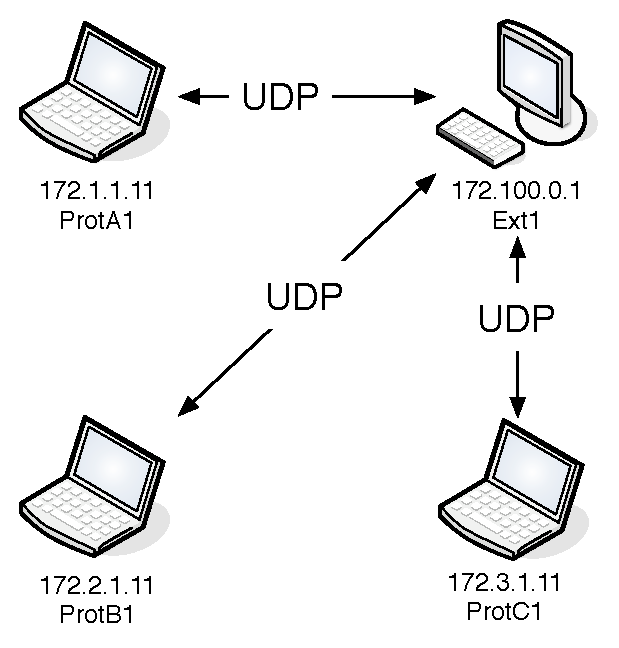
\includegraphics[height=.7\textheight]{test_traffic_0}
			\end{figure}
		\end{column}
		\begin{column}{.5\textwidth}
			\begin{figure}
			\caption{Traffic Flow 1}
			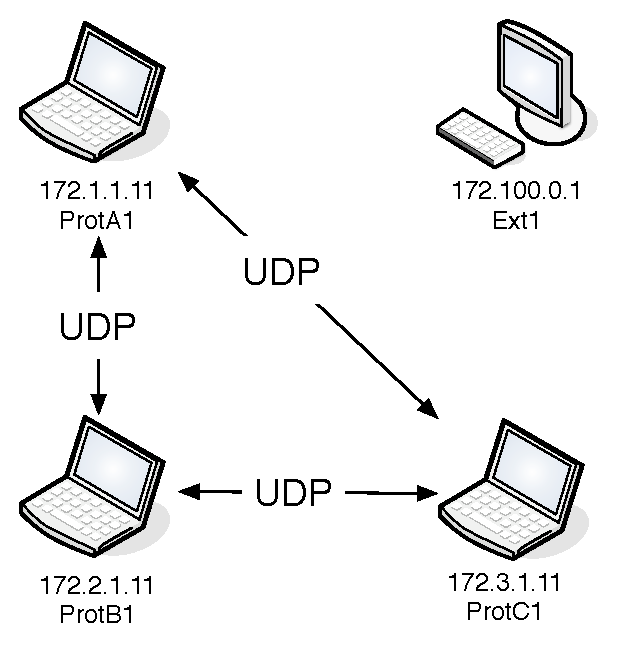
\includegraphics[height=.7\textheight]{test_traffic_1}
			\end{figure}
		\end{column}
		\end{columns}

	\onslide<2>
		\begin{columns}
		\begin{column}{.5\textwidth}
			\begin{figure}
			\caption{Traffic Flow 2}
			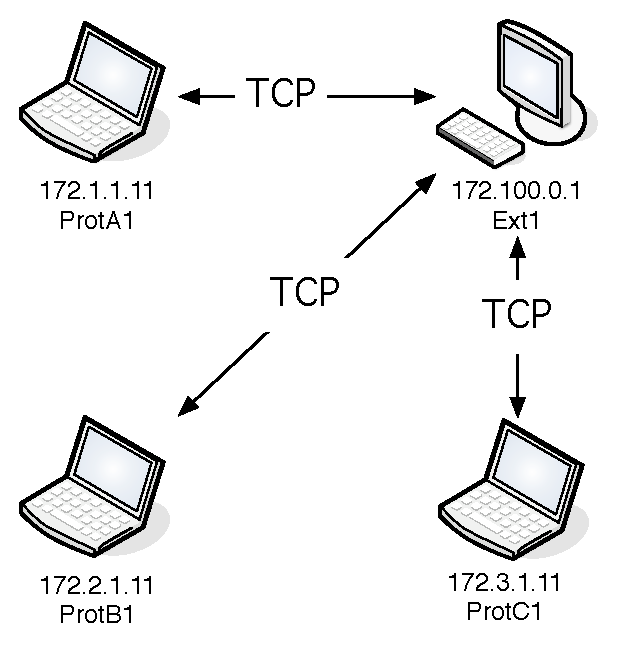
\includegraphics[height=.7\textheight]{test_traffic_2}
			\end{figure}
		\end{column}
		\begin{column}{.5\textwidth}
			\begin{figure}
			\caption{Traffic Flow 3}
			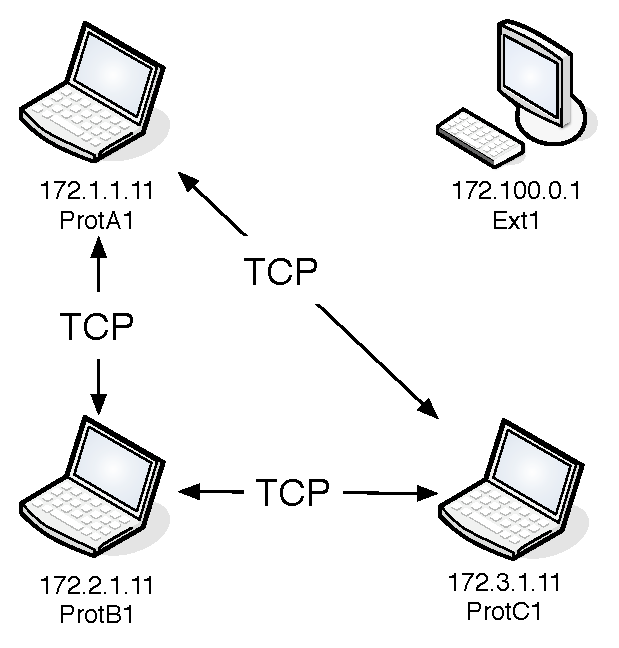
\includegraphics[height=.7\textheight]{test_traffic_3}
			\end{figure}
		\end{column}
		\end{columns}

	\onslide<3>
		\begin{columns}
		\begin{column}{.5\textwidth}
			\begin{figure}
			\caption{Traffic Flow 4}
			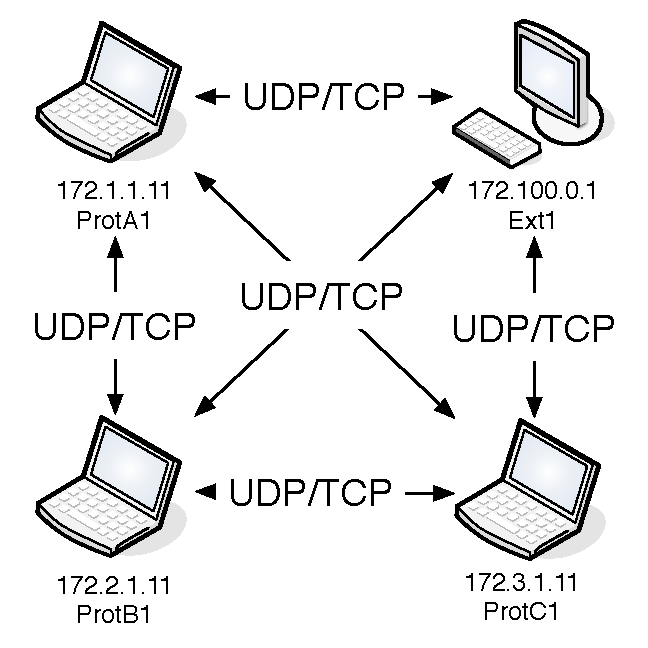
\includegraphics[clip=true,trim=5pt 0 0 0,height=.7\textheight]{test_traffic_4}
			\end{figure}
		\end{column}
		\begin{column}{.5\textwidth}
			\begin{figure}
			\caption{Traffic Flow 5}
			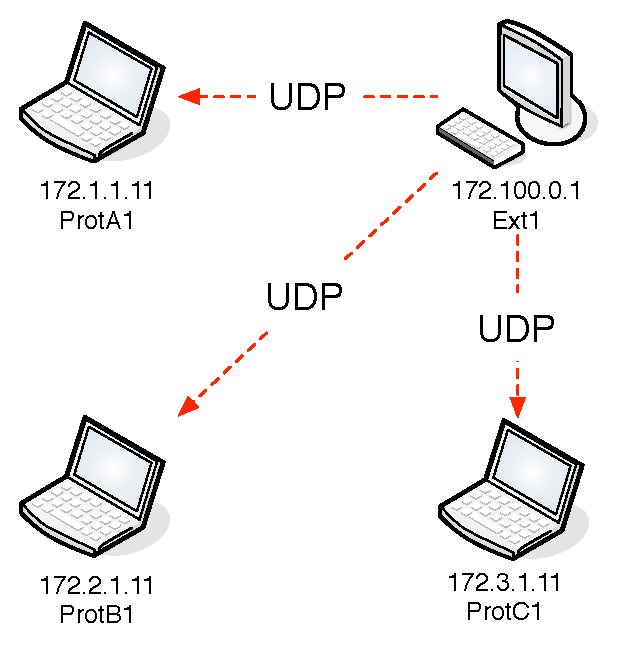
\includegraphics[height=.7\textheight]{test_traffic_5}
			\end{figure}
		\end{column}
		\end{columns}

	\onslide<4>
		\begin{columns}
		\begin{column}{.5\textwidth}
			\begin{figure}
			\caption{Traffic Flow 6}
			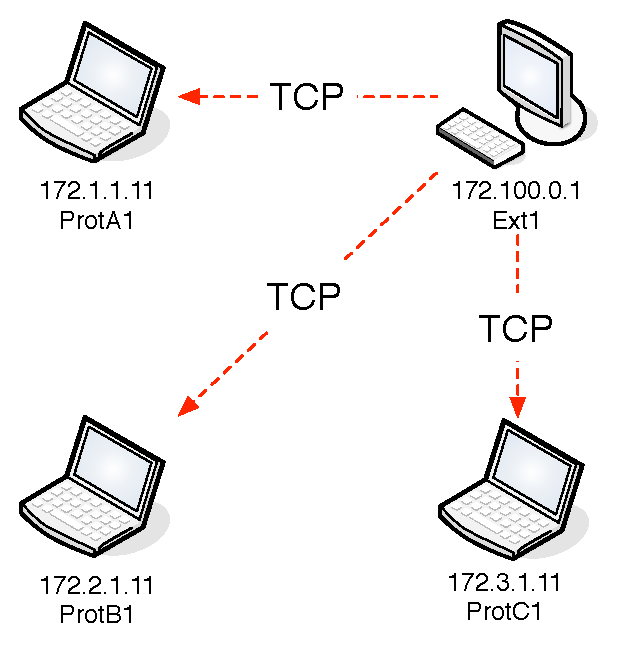
\includegraphics[height=.7\textheight]{test_traffic_6}
			\end{figure}
		\end{column}
		\begin{column}{.5\textwidth}
			\begin{figure}
			\caption{Traffic Flow 7}
			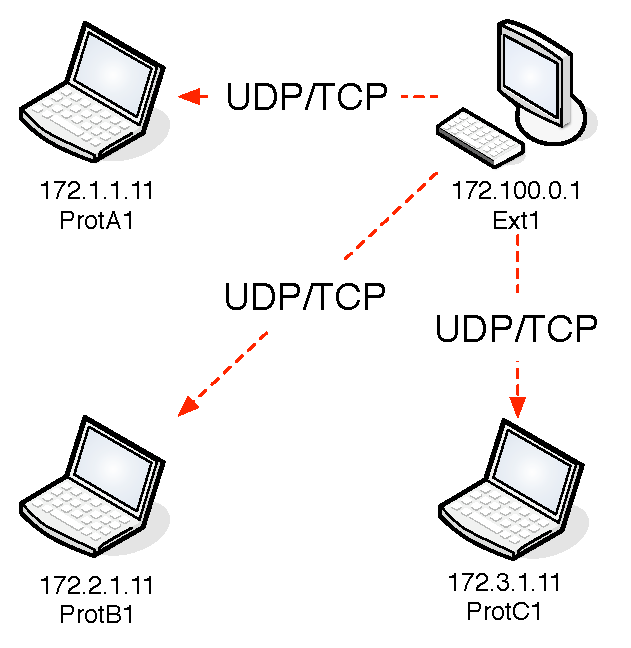
\includegraphics[height=.7\textheight]{test_traffic_7}
			\end{figure}
		\end{column}
		\end{columns}

	\onslide<5>
		\vspace{15pt}
		\begin{figure}
		\caption{Traffic Flow 8}
		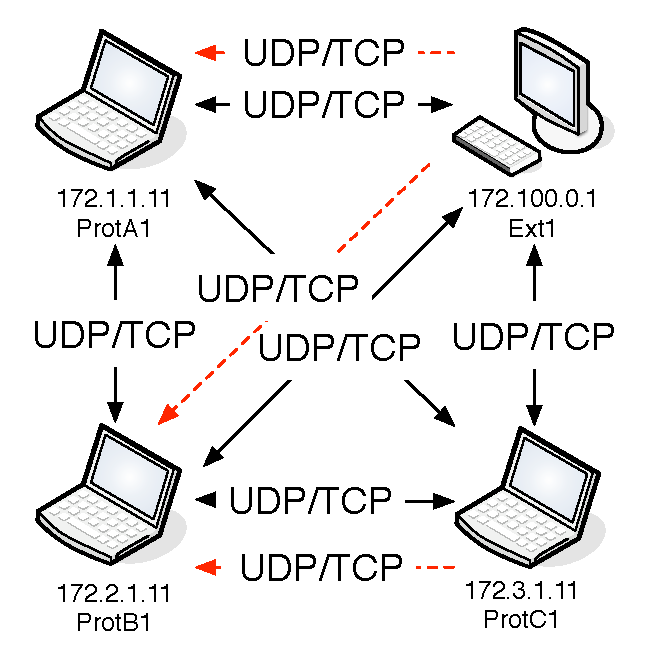
\includegraphics[height=.7\textheight]{test_traffic_8}
		\end{figure}
	\end{overprint}
\end{frame}

\begin{frame}
	\frametitle{Methodology - Test Sequences}
	
	\begin{overprint}
	\onslide<1>
		Testing broken into four sequences to focus on each research question
	
		\begin{itemize}
		\item Basic tests
		\item Maximum throughput
		\item Minimum hop interval
		\item Fuzzer
		\end{itemize}
	
	\onslide<2>
		\textbf{Basic tests} - Validate basic functionality of ARG by exercising every traffic flow

		\begin{table}
		\caption{Factor levels for basic tests}
		\label{tbl:basic_factors}
		\centering
		\begin{tabular}{ll}
		\toprule
		\textbf{Factor} & \textbf{Possible Levels} \\
		\hline
		Hop interval (ms) & 500, 50\\
		Round-trip latency (ms) & 20\\
		Packet delay (s) & 0.3\\
		Traffic direction and type & Flows 0--8\\
		\bottomrule
		\end{tabular}
		\end{table}

	\onslide<3>
		\textbf{Maximum throughput} - Test the maximum traffic rate ARG can handle

		\begin{table}
		\caption{Factor levels for throughput tests}
		\label{tbl:throughput_factors}
		\centering
		\begin{tabular}{ll}
		\toprule
		\textbf{Factor} & \textbf{Possible Levels} \\
		\hline
		Hop interval (ms) & 500, 50\\
		Round-trip latency (ms) & 20\\
		Packet delay (s) & 0.2, 0.1, 0.05, 0.01, 0.005, 0.001\\
		Traffic direction and type & Flow 4\\
		\bottomrule
		\end{tabular}
		\end{table}

	\onslide<4>
		\textbf{Minimum hop interval} - Test the maximum supportable hop rate with loss below 2\%

		\begin{table}
		\caption{Factor levels for minimum hop interval tests}
		\label{tbl:hoprate_factors}
		\centering
		\noindent\makebox[\textwidth]{%
		\begin{tabular}{ll}
		\toprule
		\textbf{Factor} & \textbf{Possible Levels} \\
		\hline
		Hop interval (ms) & 1000, 500, 300, 200, 100, 75\\
						  & 60, 50, 40, 30, 15, 10, 5\\
		Round-trip latency (ms) & 0, 30, 100, 500\\
		Packet delay (s) & 0.3\\
		Traffic direction and type & Flow 4\\
		\bottomrule
		\end{tabular}}
		\end{table}

	\onslide<5>
		\textbf{Fuzzer} - Replay traffic with 0 or more  of 7 possible modifications

		\begin{table}
		\caption{Factor levels for fuzz tests}
		\label{tbl:fuzz_factors}
		\centering
		\begin{tabular}{ll}
		\toprule
		\textbf{Factor} & \textbf{Possible Levels} \\
		\hline
		Hop interval (ms) & 500, 50\\
		Round-trip latency (ms) & 20\\
		Packet delay (s) & 0.3\\
		Traffic direction and type & Flow 8\\
		\bottomrule
		\end{tabular}
		\end{table}
	\end{overprint}
\end{frame}

\section{Results}
\begin{frame}
	\frametitle{Results - Basic Tests}

	\begin{overprint}
	\onslide<1>
		\begin{figure}
		\caption{Mean and 95\% CI for valid traffic in basic tests. Overall mean loss of .11\%.}
		\vspace{-20pt}
		\includegraphics[height=.8\textheight]{basic_tests_valid_mean}
		\end{figure}

	\onslide<2>
		\footnotesize{
		\begin{table}
		\caption{Basic tests 1-4 packet rejection reasons. 143 tests with 2,312,228 total packets represented.}
		\label{tbl:basic_loss_reasons_valid}
		\centering
		\begin{tabular}{lcc}
		\toprule
		\textbf{Reason} & \textbf{Count}  & \textbf{\% of Total Packets}\\
		\hline
		\textcolor{red}{Outbound message too long} & 949 & 0.04104\%\\
		Outbound sequence number incorrect* & 596 & 0.02578\%\\
		\textcolor{blue}{Inbound unwrapped} & 578 & 0.025\%\\
		\textcolor{blue}{Unknown} & 518 & 0.0224\%\\
		Outbound gateway not connected* & 393 & 0.017\%\\
		Inbound NAT bucket not found & 173 & 0.007482\%\\
		Inbound gateway not connected* & 78 & 0.003373\%\\
		Inbound bad protocol & 57 & 0.002465\%\\
		Inbound source IP incorrect & 30 & 0.001297\%\\
		Inbound destination IP incorrect & 6 & 0.0002595\%\\
		\textcolor{blue}{Inbound ping accepted} & 3 & 0.0001297\%\\
		Lost on wire & 2 & 0.0000865\%\\
		\textcolor{blue}{Outbound rewrite} & 1 & 0.00004325\%\\
		\bottomrule
		\end{tabular}
		\end{table}
		}

	\onslide<3>
		\begin{table}
		\caption{Basic tests, packet loss of invalid traffic}
		\label{tbl:basic_invalid_loss}
		\centering
		\begin{tabular}{lccc}
		\toprule
		\textbf{Flow} & \textbf{Mean} & \textbf{CI} & \textbf{Replications}\\
		\hline
		Flow 5 & 100\% & (100\%, 100\%) & 28\\
		Flow 6 & 100\% & (100\%, 100\%) & 28\\
		Flow 7 & 100\% & (100\%, 100\%) & 28\\
		Flow 8 & 100\% & (99.99\%, 99.99\%) & 28\\
		\bottomrule
		\end{tabular}
		\end{table}

	\onslide<4>
		\footnotesize{		
		\begin{table}
		\caption{Basic tests 5-8 packet rejection reasons. 112 tests with 1,268,746 total packets represented.}
		\label{tbl:basic_loss_reasons_invalid}
		\centering
		\begin{tabular}{lcc}
		\toprule
		\textbf{Reason} & \textbf{Count}  & \textbf{\% of Total Packets}\\
		\hline
		Inbound NAT bucket not found & 60,884 & 4.799\%\\
		Inbound unwrapped & 687 & 0.05415\%\\
		Outbound message too long & 486 & 0.03831\%\\
		Unknown & 340 & 0.0268\%\\
		Outbound sequence number incorrect & 242 & 0.01907\%\\
		Inbound source IP incorrect & 14 & 0.001103\%\\
		Inbound ping accepted & 5 & 0.0003941\%\\
		\bottomrule
		\end{tabular}
		\end{table}
		}
	\end{overprint}
\end{frame}

\begin{frame}
	\frametitle{Results - Minimum Hop Interval}

	\begin{overprint}
	\onslide<1>
		\begin{figure}
		\caption{Hop interval tests, packet loss of UDP and TCP traffic between ARG networks. Note: X axis is not linear.}
		\vspace{-20pt}
		\includegraphics[height=.8\textheight]{hop_rate_udptcp_interarg}
		\end{figure}
		
	\onslide<2>
		\begin{figure}
		\caption{Hop interval tests, scaled view of packet loss between ARG networks}
		\vspace{-20pt}
		\includegraphics[height=.8\textheight]{hop_rate_udptcp_interarg_scaled}
		\end{figure}

	\onslide<3>
		\footnotesize{
		\begin{table}
		\caption{Hop interval test loss reasons. 612 tests with 15,387,651 total packets represented.}
		\label{tbl:hoprate_loss_reasons}
		\centering
		\begin{tabular}{lcc}
		\toprule
		\textbf{Reason} & \textbf{Count}  & \textbf{\% of Total Packets}\\
		\hline
		Inbound destination IP incorrect & 506,075 & 3.289\%\\
		Inbound source IP incorrect & 165,656 & 1.077\%\\
		Inbound unwrapped & 4,935 & 0.03207\%\\
		Unknown & 4,235 & 0.02752\%\\
		Outbound message too long & 4,106 & 0.02668\%\\
		Outbound sequence number incorrect & 2,180 & 0.01417\%\\
		Outbound gateway not connected & 1,000 & 0.006499\%\\
		Inbound NAT bucket not found & 110 & 0.0007149\%\\
		Inbound bad protocol & 94 & 0.0006109\%\\
		Inbound gateway not connected & 14 & 0.00009098\%\\
		Outbound wrapped & 12 & 0.00007798\%\\
		Inbound ping accepted & 10 & 0.00006499\%\\
		Inbound connection data received & 1 & 0.000006499\%\\
		\bottomrule
		\end{tabular}
		\end{table}
		}
	
	\onslide<4>
		\tbd{triple-latency issue}

	\end{overprint}
\end{frame}

\begin{frame}
	\frametitle{Results - Maximum Throughput}

	\begin{overprint}
	\onslide<1>
		\footnotesize{
		\begin{table}
		\caption{Packet rate clusters}
		\label{tbl:pr_clusters}
		\centering
		\begin{tabular}{cccc}
		\toprule
		\textbf{Clust} & \textbf{Mean (Kbps)}  & \textbf{Min (Kbps)}  & \textbf{Max (Kbps)} \\
		\hline
		1 & 485.1 & 300.3 & 573.7\\
		2 & 854.5 & 782 & 980.3\\
		3 & 1401 & 1190 & 1581\\
		4 & 2223 & 1969 & 2421\\
		5 & 3250 & 3243 & 3264\\
		6 & 3796 & 3778 & 3814\\
		7 & 4374 & 4351 & 4389\\
		\bottomrule
		\end{tabular}
		\end{table}
		}

	\onslide<2>
		\begin{figure}
		\caption{Packet rate tests, clustered loss verses throughput}
		\vspace{-20pt}
		\includegraphics[height=.8\textheight]{max_rate_clustered}
		\end{figure}

	\onslide<3>
		\begin{figure}
		\caption{Packet rate tests, Tukey test against clustered data}
		\vspace{-10pt}
		\includegraphics[height=.8\textheight]{max_rate_tukey}
		\end{figure}
	\end{overprint}
\end{frame}

\begin{frame}
	\frametitle{Results - Fuzzer}

	\begin{itemize}
	\item ARG remains stable throughout fuzz testing
	\item 21.8\% to 23.6\% packet loss reported by run processing script
		\begin{itemize}
		\item Results not validated
		\item Cause unknown, further examination needed
		\end{itemize}
	\end{itemize}
\end{frame}

\section{Conclusions}
\begin{frame}
	\frametitle{Conclusions}

	\begin{itemize}
	\item \temporal<1>{\textcolor{gray}{Does ARG classify traffic correctly?}}{\textbf{Does ARG classify traffic correctly?}}{\textcolor{gray}{Does ARG classify traffic correctly?}}
		\only<1>{\par Overall, yes. Less than .15\% of valid traffic is lost on average and 100\% of invalid packets are dropped.}

	\item \temporal<2>{\textcolor{gray}{What is the maximum throughput ARG can support?}}{\textbf{What is the maximum throughput ARG can support?}}{\textcolor{gray}{What is the maximum throughput ARG can support?}}
		\only<2>{\par Testing shows ARG is capable of supporting at least 4 Mbps. No trend indicates this is the upper limit, however.}

	\item \temporal<3>{\textcolor{gray}{What is the minimum supportable time between hops? How does latency affect this?}}{\textbf{What is the minimum supportable time between hops? How does latency affect this?}}{\textcolor{gray}{What is the minimum supportable time between hops? How does latency affect this?}}
		\only<3>{\par The hop interval must exceed two times the round-trip latency to allow for consistent communication. 50 to 75 milliseconds appears to be a hard lower limit on the hop interval.}

	\item \temporal<4>{\textcolor{gray}{Is ARG stable when presented with corrupt, malformed, or replayed packets?}}{\textbf{Is ARG stable when presented with corrupt, malformed, or replayed packets?}}{\textcolor{gray}{Is ARG stable when presented with corrupt, malformed, or replayed packets?}}
		\only<4>{\par ARG remains stable, but exhibits high packet loss. More exploration is needed to learn why.}
	\end{itemize}
\end{frame}

\section{Future Work}
\begin{frame}
	\frametitle{Future Work}

	\begin{itemize}
	\item IPv6 support
	\item Fragmentation support
	\item More extensive malicious testing
	\item Integration with other defenses
		\begin{itemize}
		\item IDS
		\item Honeypot
		\end{itemize}
	\item Latency compensation
		\begin{itemize}
		\item Slows hops for high-latency connections
		\item Send ``in the future''
		\end{itemize}
	\end{itemize}
\end{frame}

\section{Summary}
\begin{frame}
	\frametitle{Summary}
	\tableofcontents
\end{frame}

\section{Questions}
\begin{frame}
	\frametitle{Questions}
	? \tbd{picture}
\end{frame}


%%%%%%%%%%%%%%%%%%%%%%%%%%%%%%%%%%%%%%%%
% Extra slides
\begin{frame}
	\frametitle{Late Packet Example}

	\begin{figure}
	\caption{Gateway behavior when latency exceeds the hop interval}
	\vspace{-5pt}
	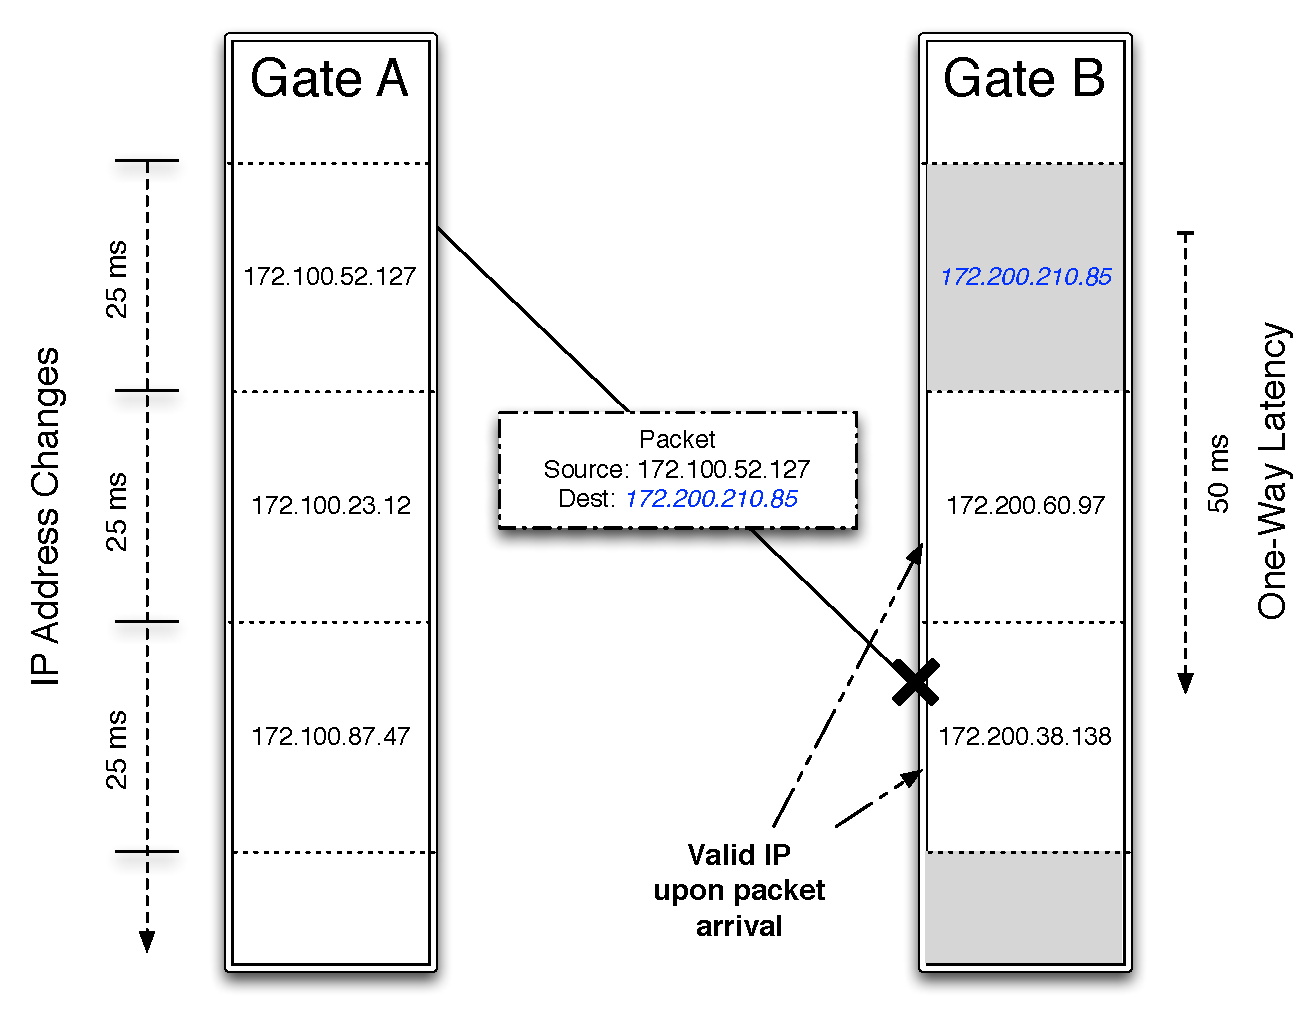
\includegraphics[height=.8\textheight]{late_packet_example}
	\end{figure}
\end{frame}

\begin{frame}
	\frametitle{Incoming Packet Validation}
	\begin{figure}
	\includegraphics[height=.8\textheight]{flow_packet_validation}
	\end{figure}
\end{frame}

\begin{frame}
	\frametitle{Fuzzer Modifications}
	
	Each chosen with 10\% probability, multiple possible
	\begin{itemize}
	\item Zero ARG signature/HMAC
	\item Change message type
	\item Zero data
	\item Remove the data
	\item Changed sequence number
	\item Changed source IP address
	\item Changed destination IP address
	\end{itemize}
\end{frame}

%\section{Lessons Learned}
\begin{frame}
	\frametitle{Lessons Learned}
	Begin full pilot studies earlier
	\begin{itemize}
	\item Discover performance problems with results processing earlier
	\item See need to run more fine-grained hop intervals at higher end
	\end{itemize}
\end{frame}

\end{document}
